\chapter{Neural Networks}
This chapter will focus on neural networks and how they were utilized for parts of this
report. First, some theoretical background surrounding neural networks in general, and then
more specifically, convolutional neural networks, is given in sections \ref{sec:NNwork}
and \ref{sec:CNN}.
Afterwards, the chapter goes more into how neural networks were tried and used during this project. Data collection and augmentation is described in sections \ref{sec:NNdata} and \ref{sec:NNaugment}. Further sections, \ref{sec:NNclassification} \& \ref{sec:NNtransfer}, describe how this data was used to train neural networks, with the latter section explaining an alternative to training a model from scratch. 
\section{How neural networks work}
\label{sec:NNwork}
There exists many different machine learning techniques out there today. Due to its high 
effectiveness and relevance, for this report we are going to focus on the highly popular 
method of artificial neural networks.
A variant, convolutional neural networks, is a proven method for working well with 
images and is therefore highly relevant for this project.

\subsection{Perceptron}
A perceptron is the simplest form of the neural network. It has a set of inputs and an output.
The perceptron first sums up all the input values, $x$, multiplied with the weight value, $w$.
After that it passes that sum through an activation function. This activation function can be everything from a simple $f(x)=x$ to the more complex sigmoid function, depending on the need. More on this in section \ref{subsec:activationfunctions}.

\begin{figure}[hbtp]
\begin{center}
\includegraphics[width = 0.75\textwidth]{./Images/perceptron.jpg} 
\caption{An illustration of the perceptron, the simplest version of a neural network.}
\end{center}
\end{figure}

A bias also exists in every node which is not based on any input. The bias function in the perceptron is similar to what the $m$ in $y = kx + m$ does. It gives the function the ability to move up and down in the graph for more possibilities of splitting the data set. The bias is usually disregarded when illustrating the perceptron.

The perceptron only has the ability to draw a single line and thus is only able to split simple data sets.

The output of the perceptron is described by the following formula:

\[ y = b + \displaystyle\sum_{i=1}^{n} x_i \cdot w_i \]

where $b$ is the bias value, $x$ is the input, $w$ is the weight for that input and $n$ is the number of inputs.

\subsection{Activation functions}
\label{subsec:activationfunctions}
The activation function,  $ \phi (v_{i}) $ , takes the sum of all the inputs from a node as input and passes them through a function before giving an output. This is beneficial when for instance the output should be kept in a range between 0 and 1, or perhaps when negative values don't make sense.
Usually, activation functions are attributed to layers instead of individual nodes.

A few commonly used functions are \textbf{ReLu}, \textbf{Tanh}, \textbf{Sigmoid} and \textbf{Softmax}.

\textbf{ReLu} is described as
\[f(x) = max(0, x)\]
and is a good option when negative values should be ignored or don't make sense. 
It is also a good choice avoiding the net to become computationally heavy.

\textbf{Tanh} is the tangens hyperbolicus function and is used to output values either as -1 or 1 like a binary operator. Unlike a binary operator, tanh's derivative is always defined which makes back propagation possible.
Back propagation is described in section \ref{subSec:optimizers}

\textbf{Sigmoid} is described as 
\[\frac{e^x}{1+e^x}\]
and works like the Tanh function but keeps the values between 0 and 1 and sets y(0) = 0.5 instead.

\textbf{Softmax} is a little bit more complex. It takes a vector $v$ of dimension $n$ and turns it into a vector $\sigma(v)$ of the same dimension where $\displaystyle\sum_{i=1}^{n} \sigma_i(v) = 1 $ and each element value is between zero and one.

Each element in the array is described as below
\[ \sigma_i(v) = \frac{e^{v_i}}{\displaystyle\sum_{j=1}^{n} e^{z_k}} \]

This output is good for describing the probability for each element to be correct and is therefore commonly used
in the output layer.

\subsection{Calculating the loss}
When training the model, it will at first make a guess to what the right answer or value is based on the random initial weigh values. In the beginning, the model is usually mostly wrong and it is then important to know how wrong it was and in what direction it should go.

For this, the model uses a loss function to calculate that error. For different applications the loss function can be different.
One way to calculate the error is to simply take the predicted value and subtract it with the correct value, $ error = y_p - y_c $.

Sometimes the sign of the error is not important. Then the absolute value can 
be calculated instead. $error = |y_p - y_c| $

Another approach is the \textbf{mean squared error} which squares the difference and takes the mean value over a few predictions.
\[Error = \frac{1}{n} \cdot \displaystyle\sum_{i=1}^{n} (y_p - y_c)^{2} \]


\subsection{Optimizers}
\label{subSec:optimizers}
Once the error has been calculated, the network will make changes to itself to improve the performance by decreasing the error value. This is called backpropagation.
The principle behind backpropagation is to go backwards in the network from the output node and changing the weight values, $ \omega $.
The optimizers decide how the weights should change. \\

A popular method for minimizing the error is to use \textbf{Gradient Decent} which works
by, step by step, move in the negative direction that minimize the error.
The direction is determined by taking the derivative of the error function.
The new weight value is calculated accordingly. $\eta$ is a chosen parameter called the learning rate.

\[ \Delta \omega_{ik} = -\eta \frac{\delta E}{\delta \omega_{ik}} \]

\begin{center}
where the error function is
\end{center}

\[E = \frac{1}{N} \displaystyle\sum_{i=1}^{N} E(n) \]

\begin{center}
which leads to
\end{center}

\[ \Delta\omega_{ik} = \frac{1}{N}  \displaystyle\sum_{i=1}^{N} \Delta\omega_{ik}(n) \]

$ E(n) $ can be, for example, mean squared error mentioned above.
The most common form of gradient decent is called \textbf{Stochastic gradient decent}, SGD.
The difference is that SGD only evaluates on a small number of nodes/patterns and updates all the weights from that observation.

\[ \Delta\omega_{ik} = \frac{1}{P}  \displaystyle\sum_{i=1}^{P} \Delta\omega_{ik}(p) \]

\textbf{Adam}, short for Adaptive moment estimation, is another optimizer which is quite popular.
The reason is because it has been proven to be a very effective algorithm in many different use cases.

Adam is a kind of combination of using \textbf{RMSPROP} and SGD with momentum.
Without going into too much detail, SGD with momentum keeps track of which direction the the improvement is in and keeps the improvement going in that same way. The optimisation goes faster when the previous direction is the same and slower when they are different. Almost like a rolling ball that gains speed as it is rolling down hill.
RMSPROP does something similar and uses a running average of each weight value and the previous values importance can be controlled with a parameter. It also only uses the sign of the direction and not its value. Also RMSPROP has individual weights.

Adam keeps a running average of both the past gradients and the squared past gradients.
The full mathematical description of Adam is given by

\[ \omega_i (t+1) = \omega_i(t) - \eta \frac{m_i}{\sqrt{v_i} + \epsilon} \]

where

\[ m_i (t+1) = \beta_1m_i(t) + (1 - \beta_1) \frac{ \delta E(t) }{\delta\omega_i} \]

\[ v_i (t+1) = \beta_2v_i(t) + (1 - \beta_2) (\frac{ \delta E(t) }{\delta\omega_i})^2 \]

and $ \eta, \beta_1 $ and $ \beta_2 $ are adjustable parameters and $ \epsilon $ a small value to keep the equation from dividing by zero.\\

There are a lot of other optimizers such as \textbf{Adagrad}, \textbf{Adadelta}, \textbf{Nadam} etc. They all have their own advantage and use-cases. We won't go into further details about them.

\subsection{Layers}

\begin{figure}[hbtp]
\begin{center}
\includegraphics[width = 1.0\textwidth]{./Images/fully_connected.jpg} 
\caption{Two fully connected layers. One with 3 neurons and one with 2 neurons.}
\label{fig:layers}
\end{center}
\end{figure}

With more layers and more neurons the networks parameters and complexity begins to grow. So does also the training time, size of the model and the cost for doing predictions. 
Thus, these networks are capable of describing much more complex data sets. But as a result of that, the risk of overfitting, the act of describing the training data set too well so that new data sets will not get recognized, becomes much greater.
That is why a complex network is not always wanted.
In figure \ref{fig:layers} an example is given of how a network with many layers might look.

\subsection{Overfitting}
\label{overfitting}
When training a neural net, one needs to be careful not to train the model too much or overfitting is likely to happen.
Overfitting is when a model gets really good at predicting the data that it is training on but fails to predict accurately on new data.
This is because it starts to pick up too much on detail or in some instances even noise.
For this reason it fails to pick up the general trends, which is more valuable.
An illustration is given i figure \ref{fig:overfitting}

\begin{figure}[hbtp]
\begin{center}
\includegraphics[width = 1.0\textwidth]{./Images/overfitting.jpg} 
\caption{Overfitting of a dataset. On the left is a generalized trained model and on the right is an overtrained model. Image taken from OReilly.com \cite{overfitting}}
\label{fig:overfitting}
\end{center}
\end{figure}

There are a few methods that can help handle the problem of overfitting. They usually involve trying to limit the size of a small amount of weights.
The hypothesis behind this is that if a weight is much larger than the rest it also has much more influence over the final prediction. That way, a small detail in the data can have much more influence than the general trend.

One way to do this is to cut random connections between layers during epochs, usually by specifying a certain amount that is going to be cut.
This way, the model is not relying on a small number of nodes to make the correct predictions. This method is called \textbf{dropout}.

Another way is to introduce random noise on a layer during training. This works because if a node with a large weight receives noise, it will be heavily amplified and probably give a false prediction.
When doing this, Gaussian noise is usually implemented, which is basically random noise with a gaussian distribution.

To force the model to keep weights small, one way is to add a penalty to the loss for every weight based on its size. 
This is called weight regularisation and is widely used and exists in two forms, L1 and L2.
L1 simply adds the weights size multiplied with an l1 term that is chosen by the designer.
The other, L2, is to do the same but in this case square that value. This has the effect of making values over 1 even bigger and values less than 1 smaller.
In that way, it doesn't affect the loss as much as L1 when not being overtrained. L2 is also called weight decay and is the more common method of the two.

Another way to keep the values between 0 and 1 is to normalize the input to every layer. In Tensorflow, this can be done with the BatchNormalization layer. \cite{batchnormalization}

One important thing to point out is that all these methods mentioned so far are only active during training and is not doing anything when making real predictions.

If lots of training data exists, the ensemble technique could be a good way to go. This technique divides the training data into smaller sets and trains a model for every data set.
The final prediction is then an average of the predictions of all the models. This technique works because if the model is highly overtrained in a certain direction, chances are that the other networks will drown out this result by the many other models.

It is kind of like when someone has an off pitch in a big choir. If there are many other singers, this off-pitch will not be noticed very much.

The final technique is called early stopping and is based on validating the model after every 
epoch and stopping the training when the validation loss, or some other criteria, is not 
improving anymore. A graph showing when to do early stopping is given in figure \ref{fig:earlystopping}.

\begin{figure}[hbtp]
\begin{center}
\includegraphics[width = 0.75\textwidth]{./Images/early_stop.jpg} 
\caption{A graph showing when to do an early stop. The graph shows the total loss over trained epochs. Notice that the validation starts to increase again somewhere after epoch 20.}
\label{fig:earlystopping}
\end{center}
\end{figure}

 \section{Convolutional Neural Networks}
 \label{sec:CNN}
Convolutional neural networks, CNN, have been used for quite some time when it comes to deep learning and their capabilities are rather astounding, as proved by Krizhevsky et al \cite{NIPS2012_4824}.  They use layers which perform convolutions, hence it's name.  The input to a convolutional network are either 2D or 3D tensors, where the 3D alternative usually has color channels along the third dimension. Use of convolutional neural networks in image recognition  can be practical for several reasons, e.g., it can tell of spatial relationships in an image. This section has been written with reference to V. Dumolin et al \cite{convArit}. Figure \ref{fig:cnn} shows an example of how a CNN may look.
 
 \begin{figure}[hbtp]
\begin{center}
\includegraphics[width = 0.9\textwidth]{./Images/convNetwork.jpg}
\caption{Image shows the flow of a convolutional neural network from left to right. Several convolutions as well as pooling functions are done in order on the input image. The last feature map is then flattened to fit into the hidden layers, to then be classified with a softmax function. Image taken from \cite{cnnImage}}.
\label{fig:cnn}
\end{center}
\end{figure}
 
A convolutional layer performs the mathematical operation \textit{convolution} on the input tensor, which can be presented as an image. A kernel of size $k \cdot l$ slides across the input and sums pixel values that are included inside the kernel; a new image containing these sums is the output. Padding on the input can be used to account for values when the kernel is outside the input. Use of padding have an impact on the output size after the convolutional layer. Stride can also be used, which tells how much the kernel translates along an axis;  increased stride leads to subsampling. Since changes of parameters in one axis do not affect outcome in another axis it simplifies explaining CNNs by having the parameter values being the same along both axes. The more convolutional layers used in a network, the more complex shapes are detected. First layers may detect edges and corners, whereas, later layers may find features representing, for example, a car or a dog. A common addition to the layers is an activation function, commonly ReLU (which is described in section \ref{subsec:activationfunctions}). This gives faster training by only allowing for positive weights to pass the layer.

 The common types of padding is \textit{no zero}, \textit{same} and \textit{full}; examples seen in figure \ref{fig:padding}. No Zero padding involves having no padding outside of the input. This means that the kernel never goes outside of the actual image, once a side of the kernel hits the side of the input it jumps down to the next line (if stride is 1). 
 
 Same padding is used when one desires the output size of the layer to be the same as the input size. This is achieved by having a padding $p$ be $ p = \floor{\frac{k}{2}} $ for any odd kernel size $k$.
  
 With full padding one actually makes the output size larger than the input, by fully utilizing every possible combination of the kernel and the input image. This is accomplished  by having the padding $p $ be $p = k - 1$ for any kernel size $k$. 
 
 
 \begin{figure}[hbtp]
\begin{center}
\includegraphics[width = 0.3\textwidth]{./Images/noPad.png}
\includegraphics[width = 0.3\textwidth]{./Images/samePad.png}
\includegraphics[width = 0.3\textwidth]{./Images/fullPad.png} 
\caption{Different examples of padding. Grid in green is the output, grid in blue is the input, and area in shadow is the current area where the kernel is currently at. Leftmost image shows a no zero padding being used. Here the kernel size is $k = 3$, input size is $i = 4$ and the output size is  $o = 2$, i.e., smaller than input.  In the middle image same padding is used; output size is the same as input size $o = i = 5$. In the rightmost image full padding is used. Here a bigger output size than the input size is produced, $o = 7, i = 5$. Images taken from \cite{convArit}}
\label{fig:padding}
\end{center}
\end{figure}
 
 
 Another useful feature used in a lot of convolutional neural networks is pooling. Pooling layers are somewhat similar to convolutional layers in that they use a sliding window which performs an operation on the contents of the window and outputs a new value. However, the difference is that they use other functions instead of linear addition. Two common pooling functions are \textit{max pooling}, where the output is the largest value within the window, and \textit{average pooling}, where the output is the average of the components within the window.  Pooling is commonly done do reduce the size of the input. Figure \ref{fig:pooling} shows example of pooling being used.
 
 \begin{figure}[hbtp]
\begin{center}
\includegraphics[width = 0.45\textwidth]{./Images/avgPool.png}
\includegraphics[width = 0.45\textwidth]{./Images/maxPool.png}
\caption{Examples of two types of pooling. Blue grid represents input, green grid represents the output, and the shaded area is where the sliding window is located. The left image shows the use of average pooling, while the right one shows the use of max pooling.
Images taken from \cite{convArit}}
\label{fig:pooling}
\end{center}
\end{figure} 
 
When a classification is to be done in the CNN, the shape needs to be shifted to an array. This is done after the last pooling layer or convolutional layer. This array can then be passed into a hidden layer for classification.


\section{Collecting data}
\label{sec:NNdata}
When working with machine learning, big sets of data is often required for a good resulting model.
A problem with this is that it can be tricky to obtain such a large data set because it usually also requires
labels with that data to be manually put in. These labels will be used by the neural network to, during training, check if
the predicted value is correct or not.

In this project the data is sets of images of different furniture parts. These images didn't exist anywhere online, so they had to be collected by taking lots of photos. The photos contained the part in different background and from different angles. The backgrounds were mostly of typical office surroundings, although there were exceptions (example is shown in figure \ref{fig:exampleCutout}). All the photos were then resized to 256x256 pixels.
The reason for choosing a square size is because when rotating them
(this will be useful later on when augmenting data in section \ref{sec:NNaugment}) 
the images will not have any black bars on the sides nor be stretched.

For the first furniture Nolmyra, there were only 3 unique parts (excluding screws and similar parts). Therefore the model was trained to recognize 4 things; the different parts and an unknown object. The unknown label was because the object detection algorithm could detect other objects and it is then unwanted that those objects be mistaken for furniture parts. This could of course also be done by setting a threshold on the confidence value, i.e., if the model gives a confidence value under 0.8 it discards it as being an unknown object. The problem with this type is that it is much harder to distinguish parts from unknown objects. This is due to that the best model is the one that can give a close to 100\% confidence value on every prediction.

For this reason, photos of random objects were also added to the data set. Most of these photos were taken by ourselves, but some were also collected from the web. The images were placed in folders with a specific item which meant labelling them became much simpler. Just put all the images containing a certain part in the same folder.

Training a model usually requires hundreds of thousands or even millions of photos. That much data is hard to get and would take a lot of time to obtain Going around the office to snap that many photos is almost unthinkable.
However, there are other options.

\begin{figure}[hbtp]
\begin{center}
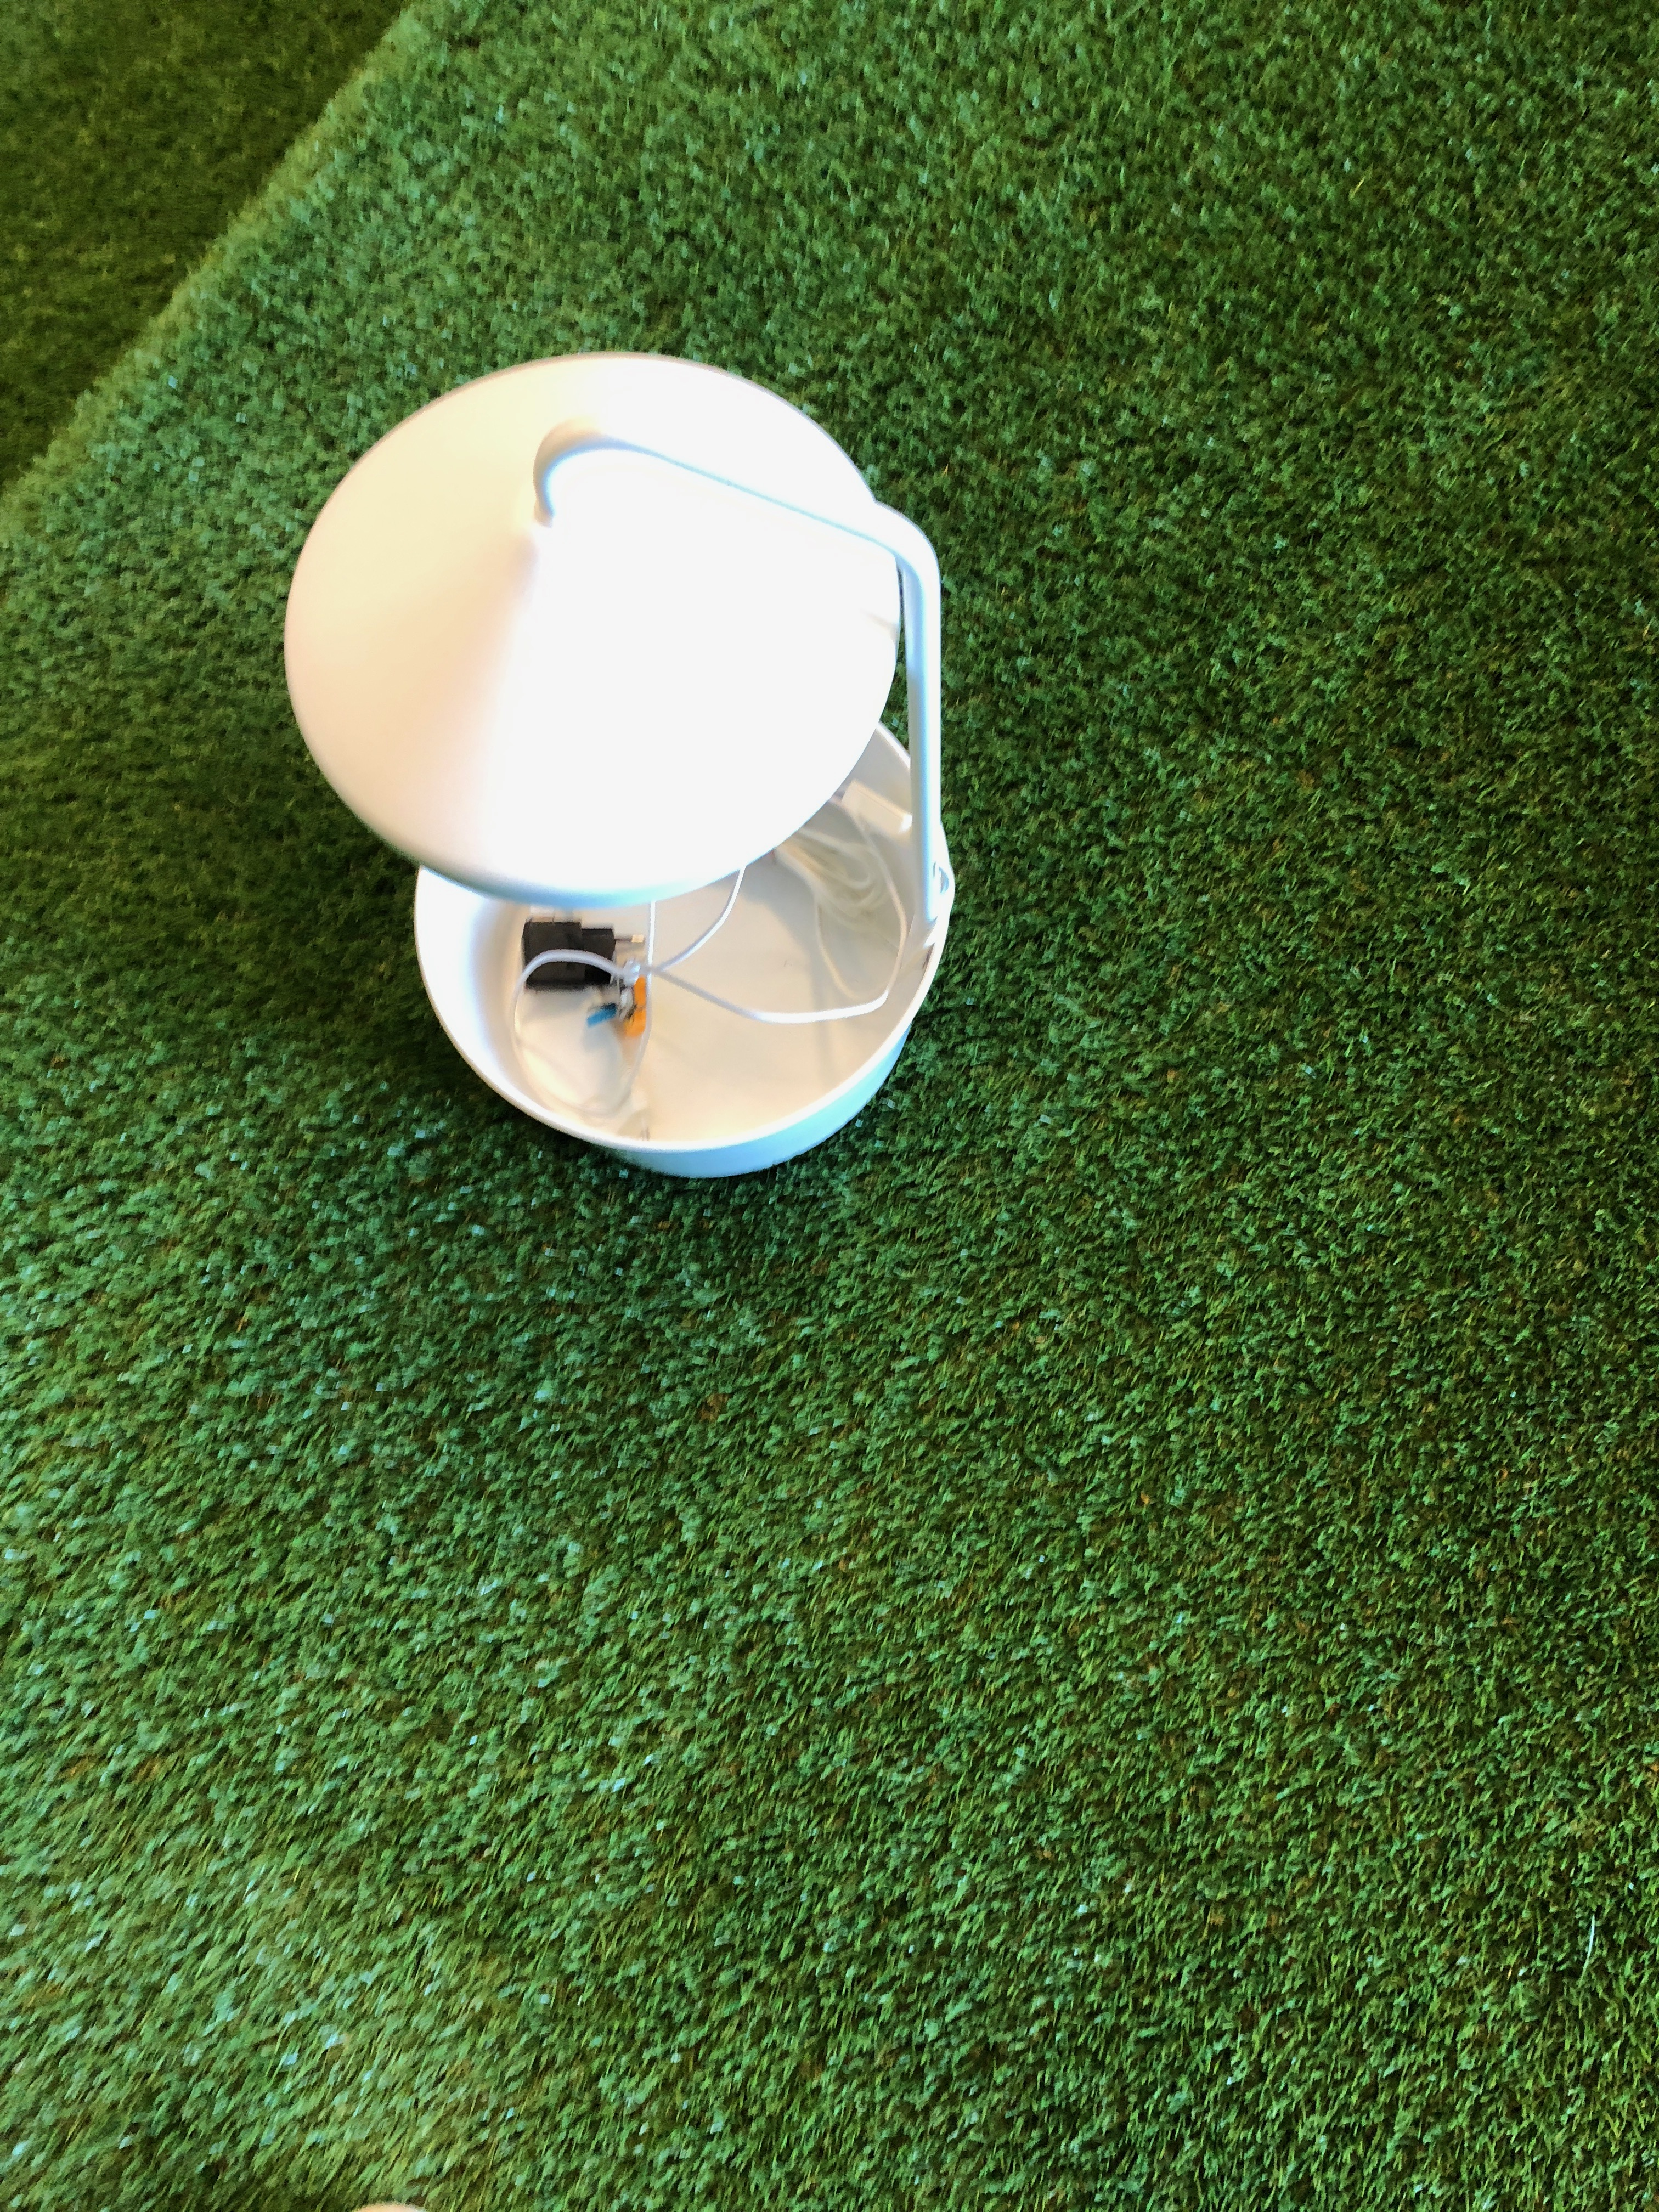
\includegraphics[width = 0.3\textwidth]{./Images/image_31.jpg}
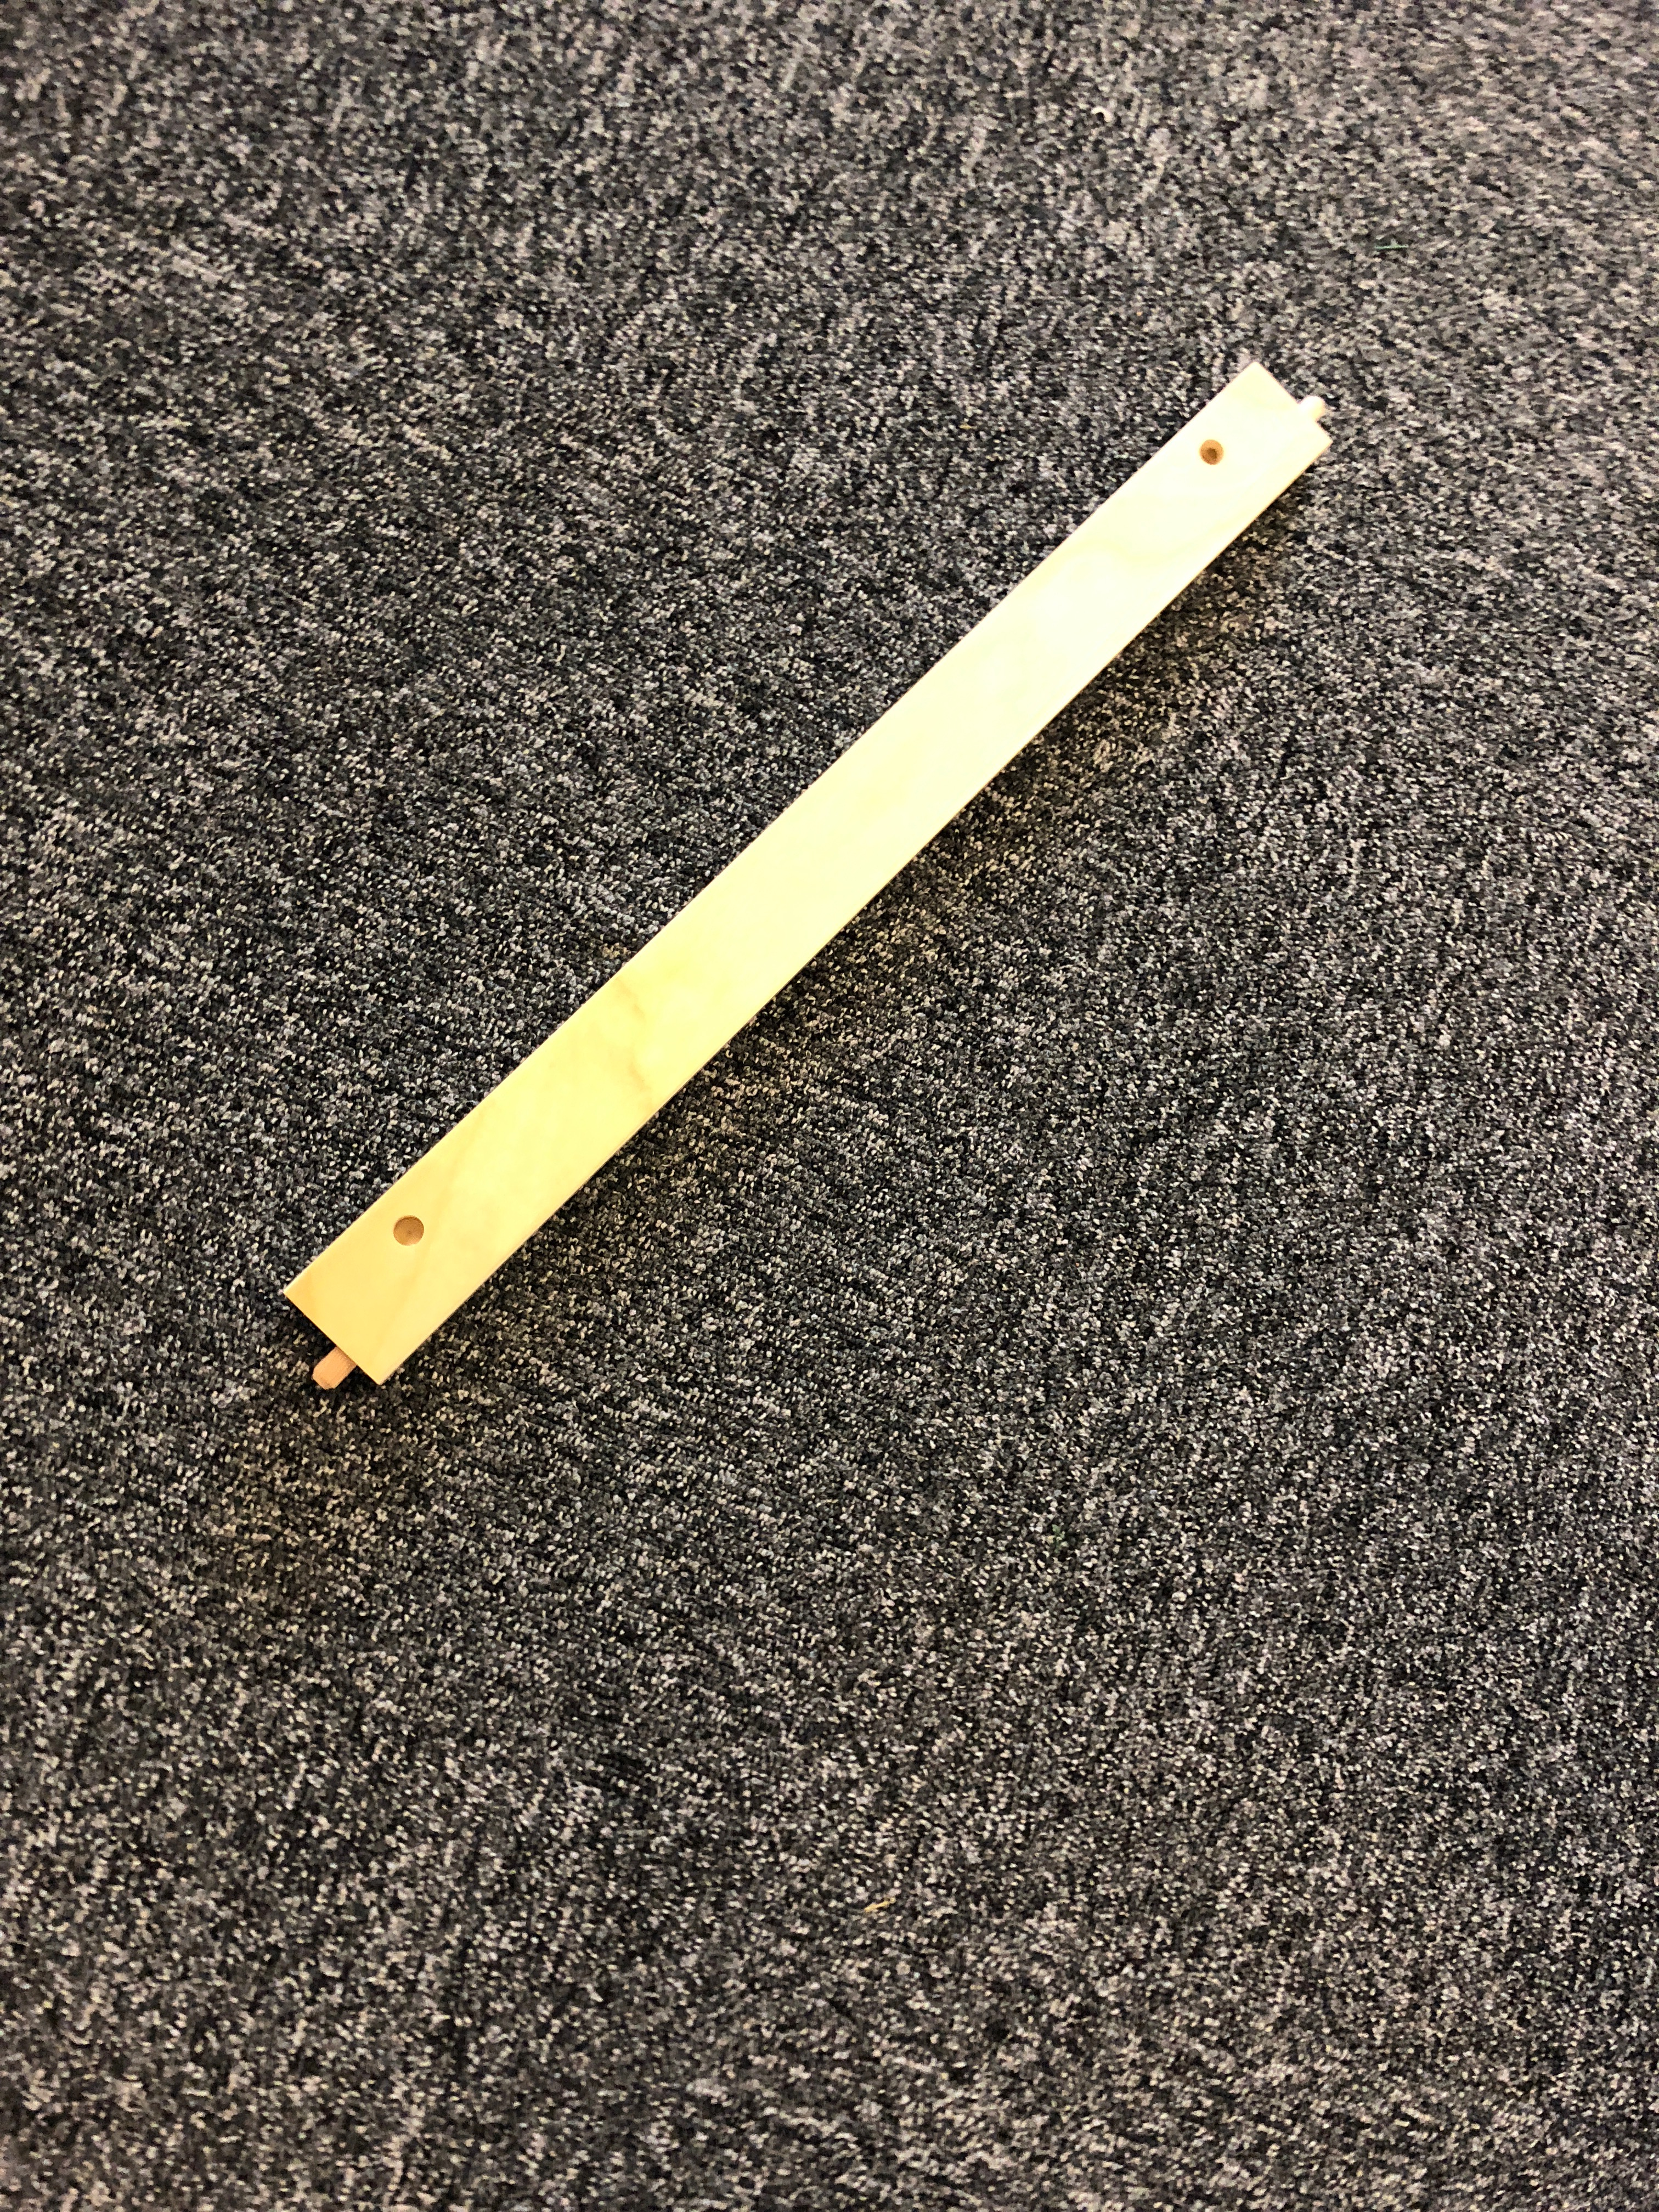
\includegraphics[width = 0.3\textwidth]{./Images/image_133.jpg}
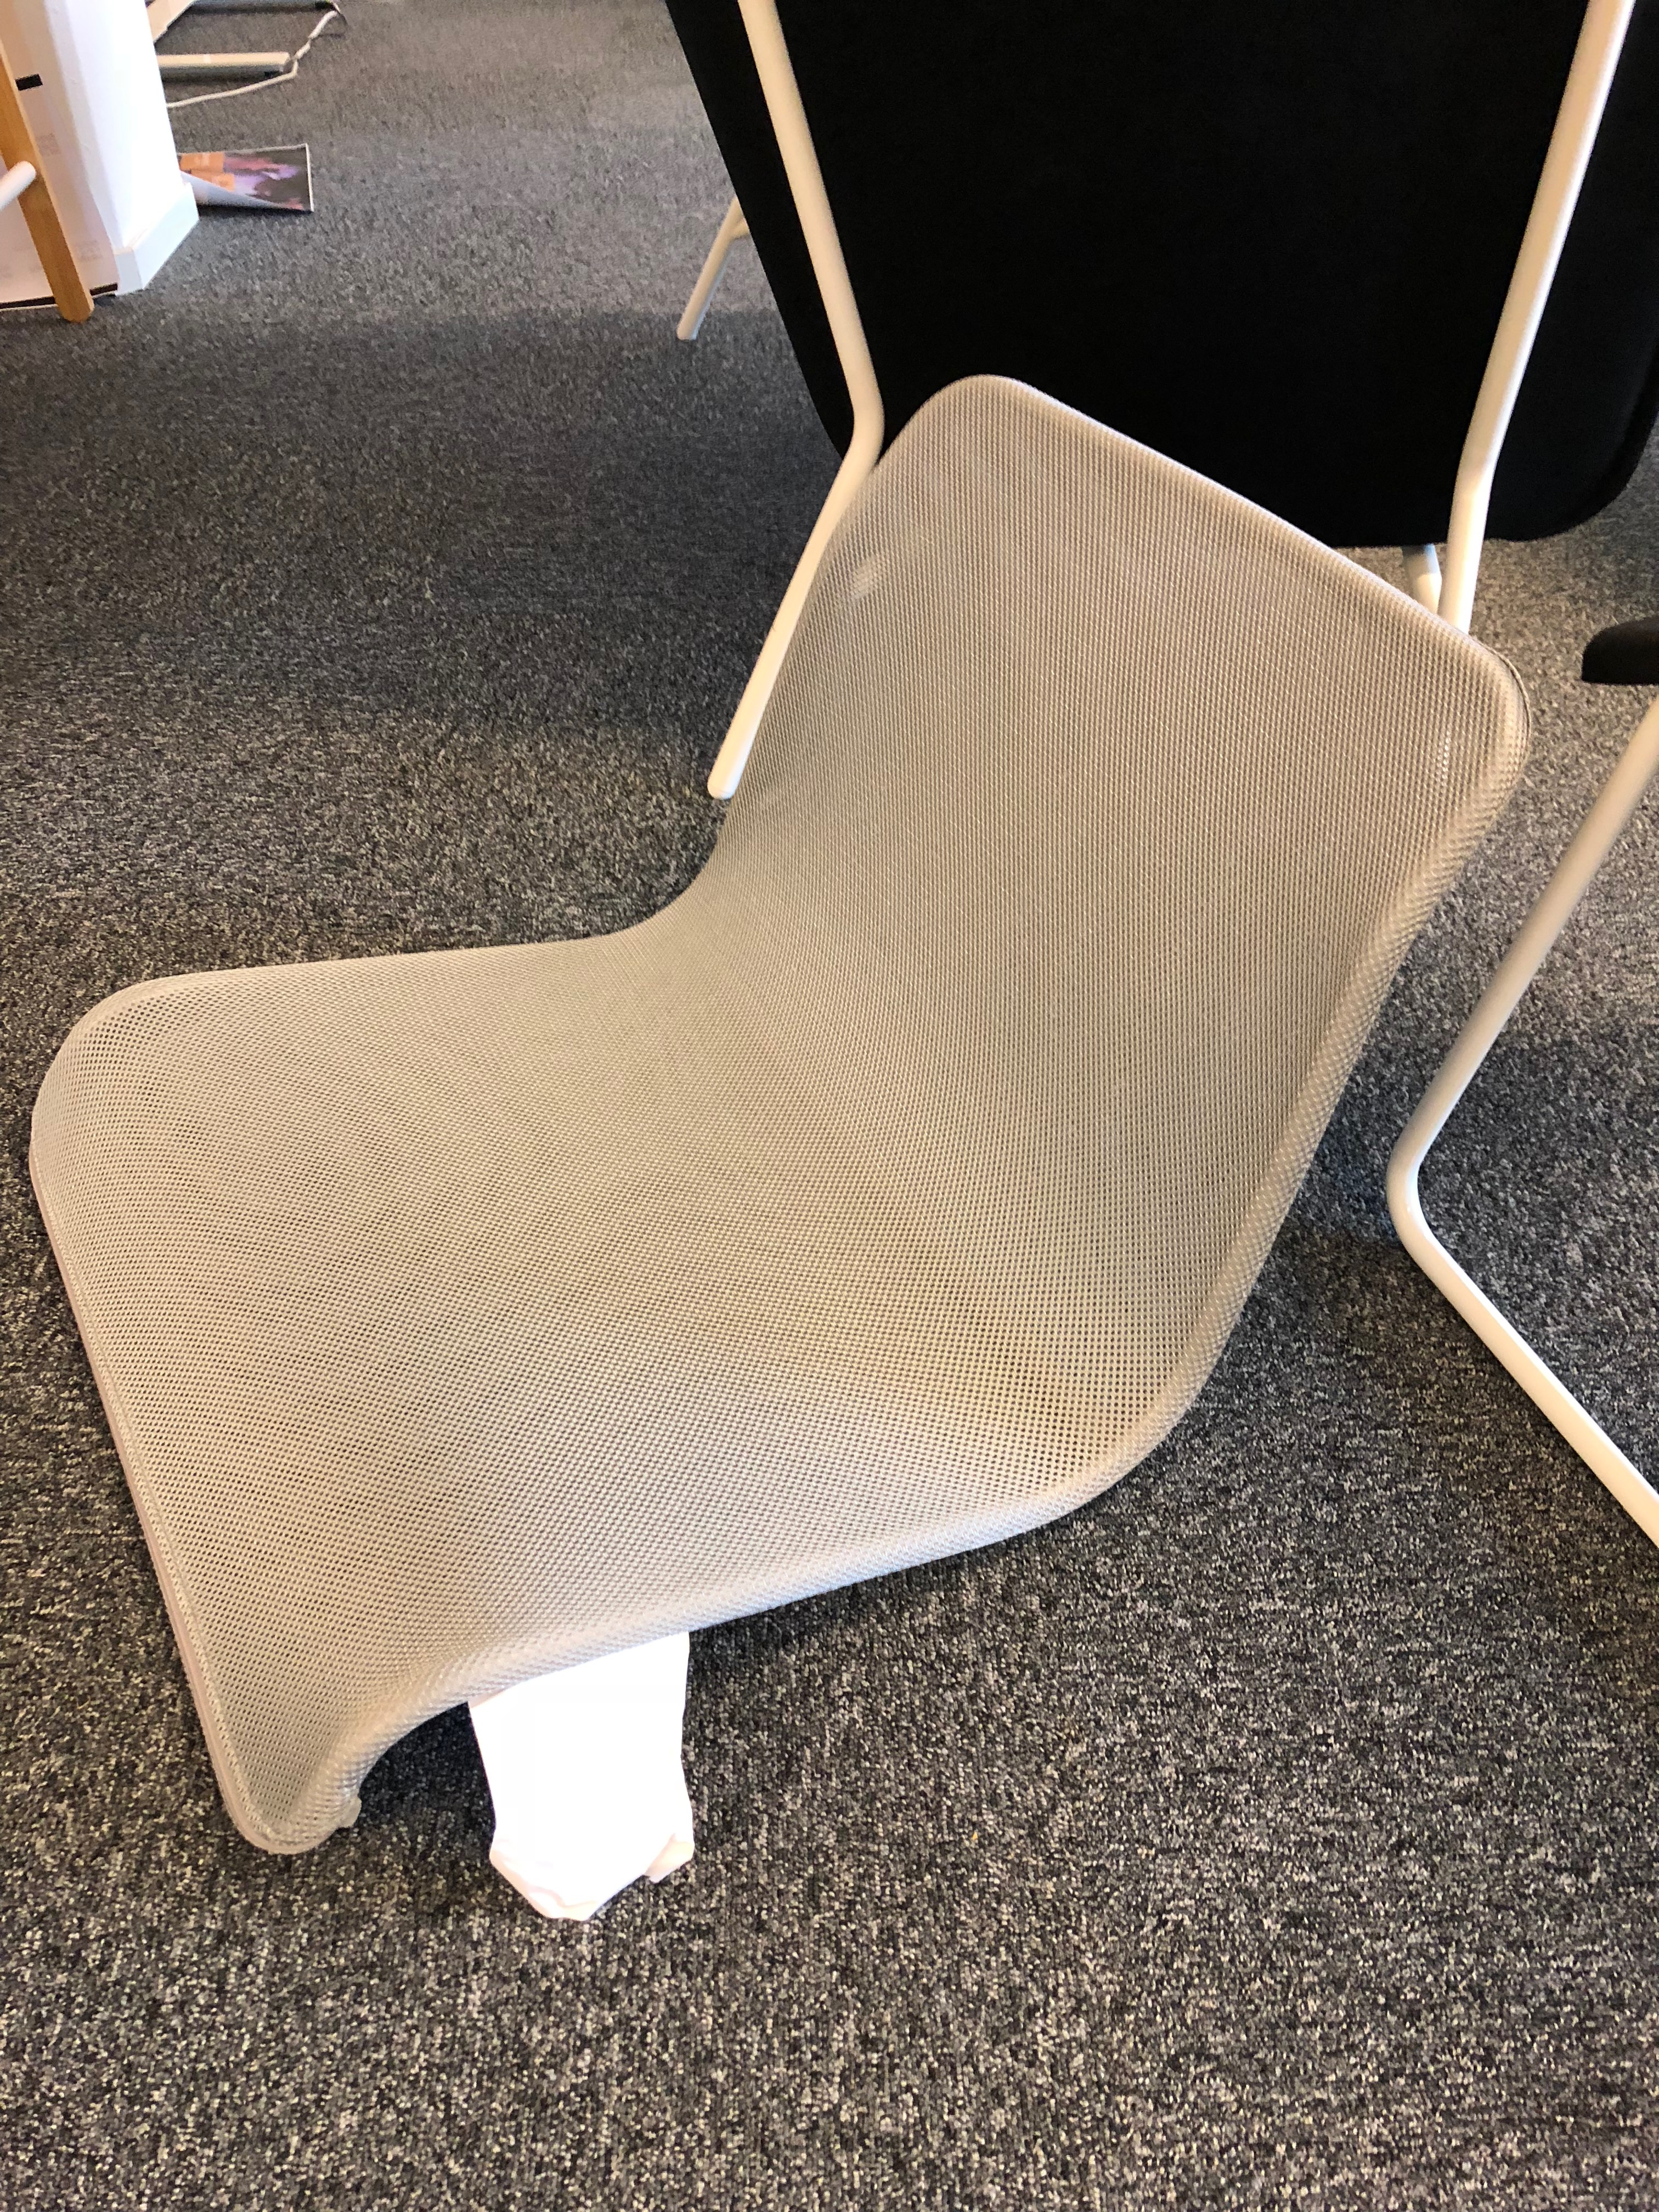
\includegraphics[width = 0.3\textwidth]{./Images/image_136.jpg}
\caption{Images showing different samples of training data used for training the model}
\label{fig:exampleData}
\end{center}
\end{figure}

\section{Augmenting data}
\label{sec:NNaugment}
Instead of training on only original images, some images can be created from other images by for example rotating, flipping, changing brightness, saturation, contrast etc.  This will essentially be an image of the same object, but the data will look different, thus giving the model more relevant data to train on, see figure \ref{fig:exampleArtificial}.
When doing this it is important to keep in mind that the augmented data should be relevant to real situations.
Creating data with only the blue color band when the real situations are only in daylight makes no sense.

\begin{figure}[hbtp]
\begin{center}
\includegraphics[width = 0.3\textwidth]{./Images/image_15-1.jpg}
\includegraphics[width = 0.3\textwidth]{./Images/image_15-3.jpg}
\includegraphics[width = 0.3\textwidth]{./Images/image_15-4.jpg}
\includegraphics[width = 0.3\textwidth]{./Images/image_15-9.jpg}
\includegraphics[width = 0.3\textwidth]{./Images/image_15-11.jpg}
\includegraphics[width = 0.3\textwidth]{./Images/image_15-12.jpg}
\caption{Images showing some resulting images from augmentation. Top left image shows the original image. Top middle image shows the result after rotating $180$ degrees. Top right image shows result after rotating $-90$ degrees. Bottom left image show result after  reducing the contrast with by $30\%$. Bottom middle image shows result after reducing color balance by $70\%$. Bottom right image shows result after increasing color balance by $60\%$.}
\label{fig:exampleArtificial}
\end{center}
\end{figure}

Furthermore, images of objects of interest can be cut out and pasted into random environments to create even more data, see figure \ref{fig:exampleCutout}.
The idea of this is to try and make the model understand that the focus should be on the furniture part and the background environment is irrelevant. While doing this, even though the parts could be cut into totally random environments we tried to focus on pasting them into relevant spaces like office floors or carpets.
In our project, this gave a good result as it increased the test accuracy by 8\%.

\begin{figure}[hbtp]
\begin{center}
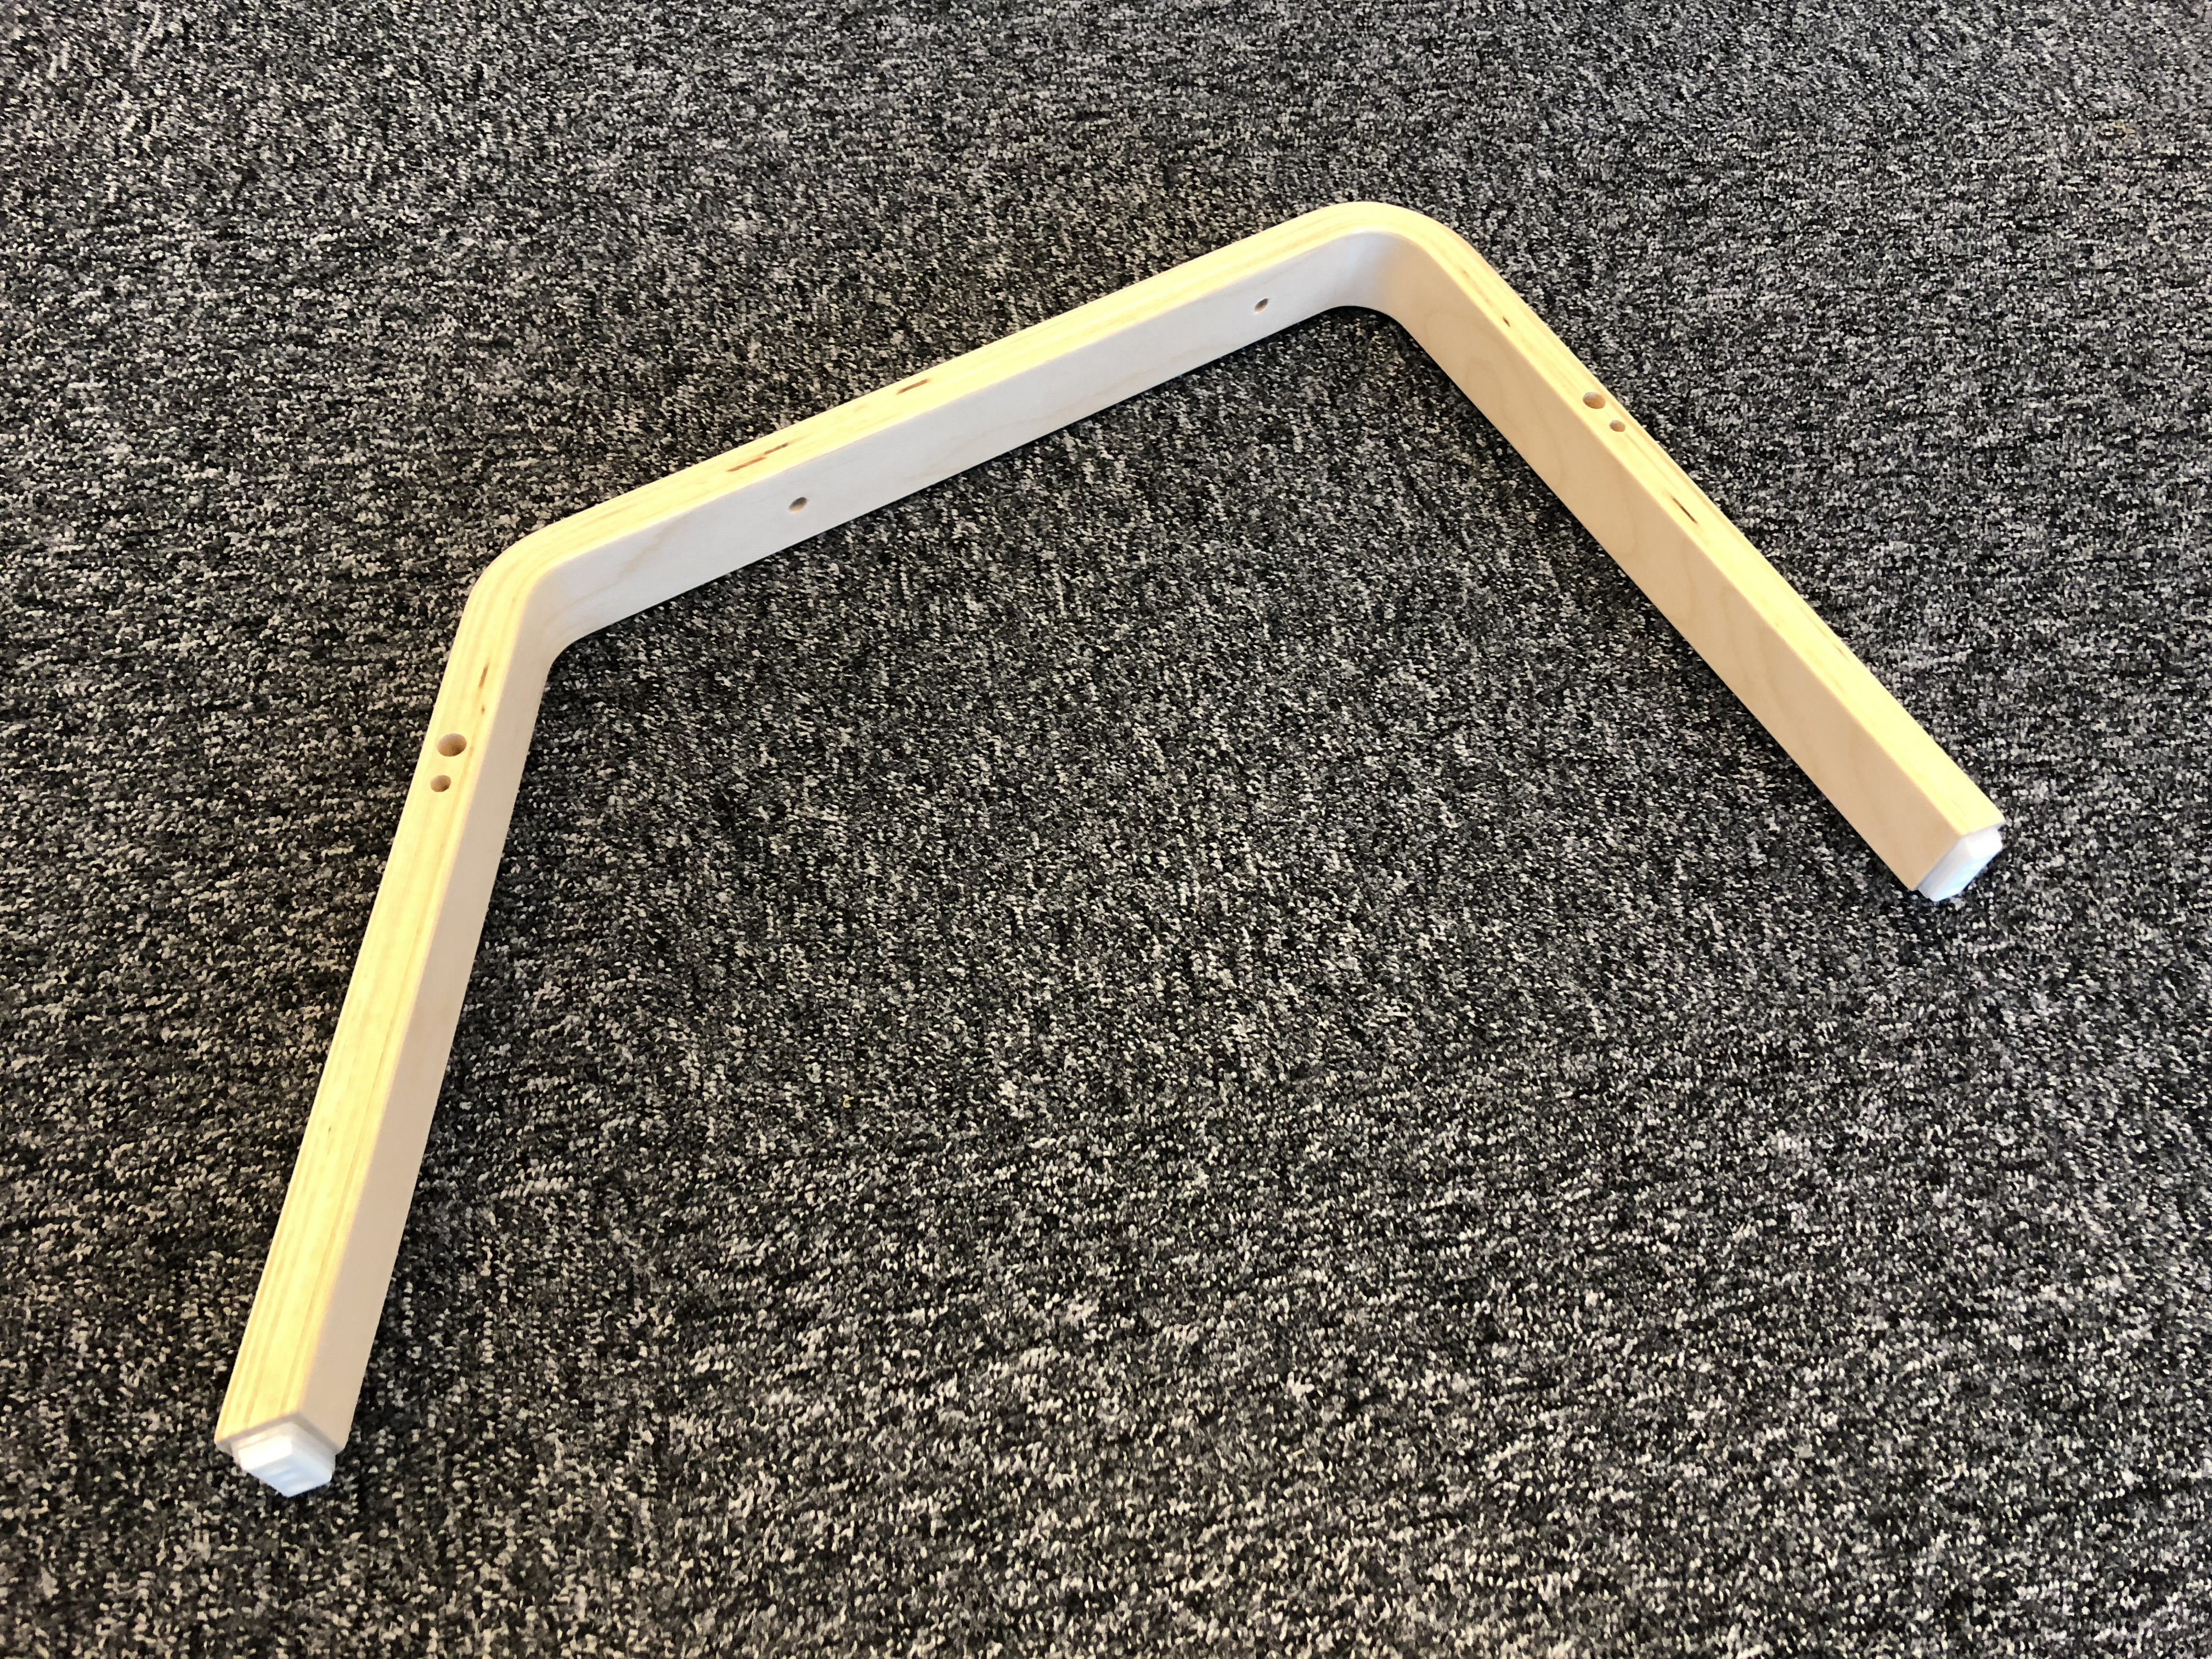
\includegraphics[width = 0.3\textwidth]{./Images/image_13.jpg}
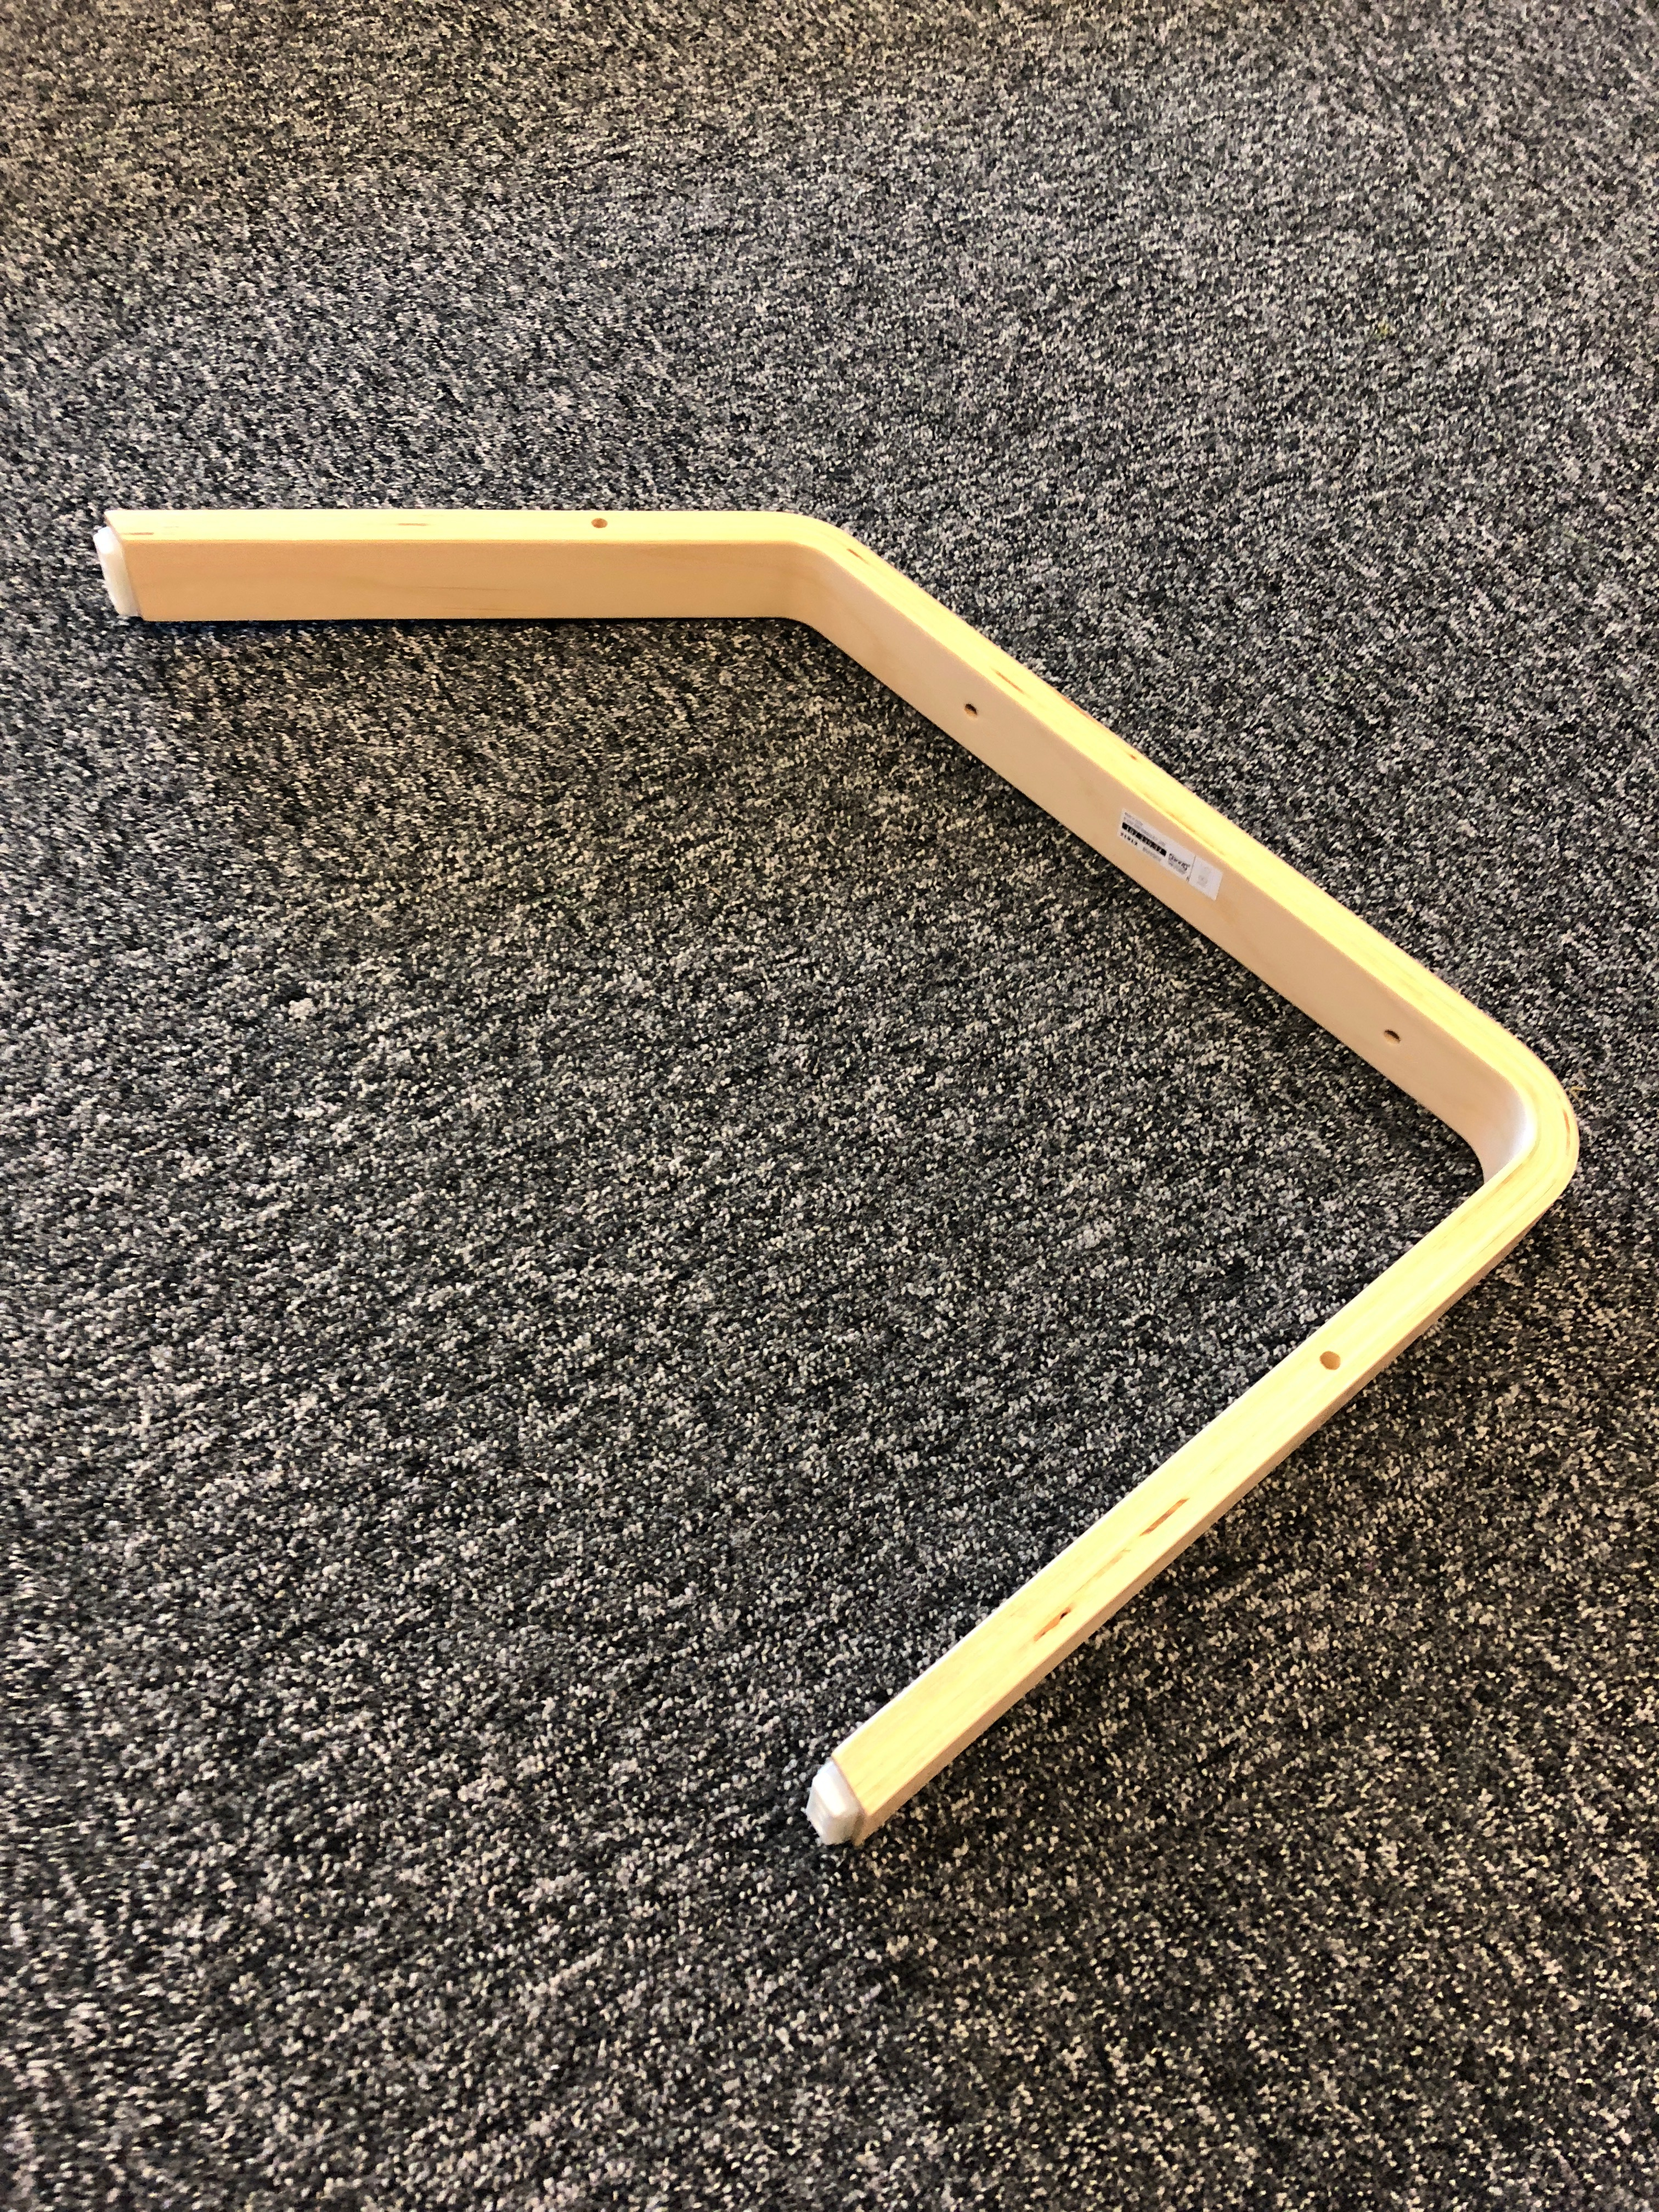
\includegraphics[width = 0.3\textwidth]{./Images/image_86.jpg}

\includegraphics[width = 0.3\textwidth]{./Images/image_107.jpg}
\caption{Images showing how cutouts of images were utilized. Leftmost image shows a cutout of one of the furniture parts. The other two images show the result after they were pasted in to different environments to artificially increase training data.}
\label{fig:exampleCutout}
\end{center}
\end{figure}


Doing this by hand can still be very time consuming, so automating this process as far as possible is recommended.

\section{Image classification}
\label{sec:NNclassification}
Designing a neural network for the image classification is not the easiest task and much
work consists of trying things and making intelligent guesses.
As stated in the section about data collection we had 4 different classes to classify,
which means that a test accuracy of over 25\% would be significant. We were aiming for
somewhere above or around 90\% with a relatively small amount of data.

We started out with many convolutional layers layered with pooling layers and a few dense
layers at the end. The final layer had four nodes and softmax activation functions to give a
classification probability between four classes.
The activation functions of the other layers were set to ReLu since they are the fastest
and preferred for larger nets. Tanh was also tried but with no success.

SGD with momentum as an optimizer was tested but was was changed to Adam
quite early on since it had better performance.
Only linear optimizers were considered because non-linear optimizers take a lot of
computing power and are usually only recommended for small networks.

We went back and forth with trying different mixes of kernel sizes, amounts of convolutional
layers, insertion of pooling layers on different places, stride sizes, amount of dense layers
and how many nodes they had.

When training the models, overfitting was a big problem from the start. The tested methods
for combating this was dropouts with different values, L2 weight regularisation,
batch normalization and reducing the number of weights.

It was hard to reduce the number of weights as the evaluation usually converged around 25\%
whenever it was tried.
When using the dropout method a value of 50\% with a minimum of 64 nodes in the layer
reduced overfitting most effectively. That, with a combination of weight regularisation and batch 
normalization gave good results. Figure \ref{fig:imageclassification} shows how overfitting was avoided.

Gaussian Noise gave very good results, but was unfortunately not possible to be 
converted from the model format generated in keras, to the mlmodel format that is required for Xcode.

The most important thing to mention is the difference the amount of photos we had and how they
were taken. Adding more photos made a huge difference to the test evaluation score.
After having added 50 more images per class with a library of 600 images the test score increased
from \textbf{80.55\%} to \textbf{83.45\%} in accuracy. \\

When finally testing the model we made a mistake by not separating the training data and test data.
Since we shuffled our data before splitting it up into two parts, some augmented data got into the
test set. The model had already trained on the original image and it was similar enough to
give unrealistic good results of 99.52\%. This was finally fixed by splitting up the test and train data 
into separate folders. Figure \ref{fig:augmentedtestdata} shows the printed graph from one of those
training sessions.

\begin{figure}[!hbtp]
\begin{center}
\includegraphics[width = 0.4\textwidth]{./Images/augmentedtestdata}
\caption{Test and train accuracy over a 100 epochs. The performance seems much better than it actually is.}
\label{fig:augmentedtestdata}
\end{center}
\end{figure}

\begin{figure}[!hbtp]
\begin{center}
\includegraphics[width = 0.4\textwidth]{./Images/imageclassification1}
\includegraphics[width = 0.4\textwidth]{./Images/imageclassification2}
\includegraphics[width = 0.4\textwidth]{./Images/imageclassification3}
\caption{Images shows the result from introducing weight regularisation and dropout to a model. The graphs show the training loss (green) and evaluation loss (red). The upper left image shows the training without any dropout or weight regularisation. The upper right image shows the training with dropout implemented. The bottom image shows the training with dropout and weight regularisation implemented.}
\label{fig:imageclassification}
\end{center}
\end{figure}

As shown in the code below, early stopping was also finally implemented with a callback to save
highest performing model at the end of the process.

\begin{lstlisting}[language=python]
#Python script from training
#Project path:
	master-thesis/Training/trainer.py
import tensorflow as tf
from tensorflow import keras
import numpy as np
import matplotlib.pyplot as plt
from PIL import Image
from sklearn.utils import shuffle

train_images = []
train_labels = []
loadImages(train_images, train_labels, "Train", 200)
train_images = reshapeArray(train_images)

test_images = []
test_labels = []
loadImages(test_images, test_labels, "Test", 39)
test_images = reshapeArray(test_images)

# Create the neural network
model = keras.Sequential([
	keras.layers.Conv2D(4, kernel_size=(5, 5), strides=(2, 2), input_shape=(image_height, image_width, number_of_color_channels)),
		
	["The code for the hidden layers"]

	keras.layers.Dense(4, activation=tf.nn.softmax)
])

model.compile(optimizer=keras.optimizers.Adam(),
	    loss='sparse_categorical_crossentropy',
	    metrics=['accuracy'])
	    
train_data, train_labels = shuffle(train_data, train_labels)

early_stopping = keras.callbacks.EarlyStopping(monitor='val_acc', patience=5, verbose=1)
checkpoint = keras.callbacks.ModelCheckpoint("./Models/Nolmyra.h5", monitor='val_acc', 
verbose=1, save_best_only=True, save_weights_only=False, mode='auto', period=1)

history = model.fit(train_data, train_labels, epochs=40, batch_size=10, validation_data=(test_images, test_labels), callbacks=[early_stopping, checkpoint] , verbose=1)

model.save("./Models/recognizer.h5")
\end{lstlisting}

The network that proved to be the best performing network (\textbf{92.25\%} accuracy) had the following configuration:

\begin{lstlisting}[language=python]
Conv2D(4, kernel_size=(5, 5), strides=(2, 2), input_shape=(image_height, image_width, number_of_color_channels)),
Conv2D(4, kernel_size=(3, 3), strides=(1, 1), input_shape=(image_height, image_width, number_of_color_channels)),
MaxPool2D(pool_size=(2, 2), padding="valid"),
BatchNormalization(),
LeakyReLU(),
Conv2D(8, kernel_size=(3, 3), strides=(1, 1)),
Conv2D(8, kernel_size=(3, 3), strides=(1, 1)),
Conv2D(8, kernel_size=(3, 3), strides=(1, 1)),
MaxPool2D(pool_size=(2, 2), padding="valid"),
BatchNormalization(),
LeakyReLU(),
Conv2D(16, kernel_size=(3, 3), strides=(1, 1)),
Conv2D(16, kernel_size=(3, 3), strides=(1, 1)),
Conv2D(16, kernel_size=(3, 3), strides=(1, 1)),
MaxPool2D(pool_size=(2, 2), padding="valid"),
BatchNormalization(),
LeakyReLU(),
Flatten(),
Dropout(0.5),
Dense(64, kernel_regularizer=keras.regularizers.l2(0.003), activation=tf.nn.relu),
GaussianNoise(0.2),
Dense(64, kernel_regularizer=keras.regularizers.l2(0.003), activation=tf.nn.relu),
Dropout(0.25),
Dense(4, activation=tf.nn.softmax)
\end{lstlisting}

A model with many convolutional layers and a few dense layers at the end gave the best
results. A larger network could have been implemented and tests as well but
since the model size would grow more and training time would increase drastically,
we didn't increase it further.

\section{Transfer Learning}
\label{sec:NNtransfer}
% Write about how we went about in order to insert Transfer Learning into the mix. 
After trial of designing the network from scratch, it was decided to try and make use of 
pre-trained networks and then retrain them for another purpose. Models trained on 
imageNet \cite{imageNet} were chosen since that source domain is similar to this target 
domain. The models with their respective weights were loaded, without their fully 
connected layer. The top layer's weights were then frozen at different stages, and new 
fully connected layers were added on top, and new classifiers were trained. 
Several different models were tried, including ResNet50, InceptionV3 and VGG16, 
which where all integrated in Keras to start with.

Code below shows how to load the VGG16 network which has weights that has been pretrained on imageNet. The fully connected layer is then removed and instead a custom top layer is added to be trained. 
\begin{lstlisting}[language=python]
#Project path: master-thesis/FeatureTraining/transferLearning.py
from keras import applications
from keras.preprocessing.image import ImageDataGenerator
from keras import optimizers
from keras.models import Sequential, Model
from keras.layers import Dropout, Flatten, Dense, GlobalAveragePooling2D, Input, Conv2D, MaxPool2D
from keras import backend as k
from keras.callbacks import ModelCheckpoint, LearningRateScheduler, TensorBoard, EarlyStopping

#Load data and pretrained model
img_width, img_height = 256, 256
train_data_dir = "data/train"
validation_data_dir = "data/val"
nb_train_samples = 129
nb_validation_samples = 21
batch_size = 16
epochs = 50
input_layer = Input(shape=(256,256,3))
model = applications.VGG16(include_top=False, weights='imagenet', input_tensor=input_layer, pooling=None)

#Cut network and add own layers
x = model.get_layer('block5_pool').output
x = Flatten()(x)
x = Dense(512, activation="relu")(x)
predictions = Dense(4, activation="softmax")(x)

# creating the composed model
model_final = Model(inputs = model.input, outputs = predictions)
for layer in model_final.layers[:-2]:
    layer.trainable = False
    
# compile the model
model_final.compile(loss = "categorical_crossentropy", optimizer = optimizers.SGD(lr = 0.0001, momentum = 0.9), metrics=["accuracy"])

#Hidden lines of code
.........

#Train the model
hist = model_final.fit_generator(
train_generator,
epochs = epochs,
validation_data = validation_generator,
callbacks = [checkpoint, early])
\end{lstlisting}

The best result  that was achieved for each of the models using this method is listed in
 table \ref{table:transferLearning}. It shows that using InceptionV3 model with pretrained
 weights gave the best result. However, a few factors, such as, where the models were
 frozen, how adding and removing layers, has most likely affected the results. As can be
 seen from using ResNet, the best model achieved 25\% accuracy, which is the same as making a guess, seeing as there are only four possible classes. These models could, and would most like have been, improved if it was not decided to take a new approach to the problem, which is described further in section \ref{sec:ODresults}

\begin{table}[h]
\centering
\begin{tabular}{ |c|c| } 
 \hline
 Pretrained model used &  Best achieved accuracy  \\ 
 \hline
 VGG16 & 70.8\%. \\ 
 \hline
 ResNet & 25.0\% \\ 
  \hline
 InceptionV3 & 72.9\% \\ 
 \hline
\end{tabular}
\caption{Results from doing transfer learning .}
\label{table:transferLearning}
\end{table}


\newpage